% The ICIP2016 paper according to the given template
%          spconf.sty  - ICASSP/ICIP LaTeX style file, and
%          IEEEbib.bst - IEEE bibliography style file.
% --------------------------------------------------------------------------
\documentclass{article}
\usepackage{spconf,amsmath,graphicx}

% Example definitions.
% --------------------
\def\x{{\mathbf x}}
\def\L{{\cal L}}

% Title.
% ------
\title{Data-driven Region Detector for Structured Image Scenes}
%
% Single address.
% ---------------
\name{Elena Ranguelova}
\address{Netherlands eScience Center\\ Amsterdam, The Netherlands}
%
% For example:
% ------------
%\address{School\\
%	Department\\
%	Address}

%
\begin{document}
%\ninept
%
\maketitle
%
\begin{abstract}
A Data-driven Morphology Salient Regions (DMRS) detector, related to our MSSR detector is proposed.
It demonstrates comparable repeatability to the best-known MSER detector on standard structured scenes and better resolution invariance on a high-resolution benchmark. This is achieved via significantly smaller number of detected regions- a much desired property in the big data era. A data-driven binarization algorithm gives compact image representation, subsequently analyzed for saliency using morphology.  Also, a new benchmark dataset, 'OxFrei', for transformation-independent detection evaluation is introduced.
While MSER is an excellent detector for generic applications, the DMSR is geared towards the analysis of scientific imagery for detecting precisely semantically meaningful regions. This is a key property in emerging domains such as animal and plant biometrics, where computer vision becoming the vital technology to aid the wild-life preservation efforts. In this paper, DMSR is demonstrated to better detect identifying structures in marine animals and wood microscopy images.

\end{abstract}
%
\begin{keywords}
region detection, data-driven, morphology, structured scenes, scientific visual analyics
\end{keywords}
%
\section{Introduction}
\label{sec:intro}
Finding reliably and repeatedly correspondences between two images of the same object or scene, taken under different viewpoints and acquisition conditions, is the first fundamental step in numerous computer vision applications: wide baseline stereo matching, image retrieval, model-based recognition, visual mining, object categorization, etc. An important class of features are the stable and salient regions, which correspond to the same image patches for different viewpoints, detected independently for each image. The region detectors must be {\em covariant} (or often called {\em invariant} in the literature) to a class of transformations, usually {\em affinity} and various photo-metric distortions. 

While the most research has been focused on the generic applications, the emerging fields of {\em animal and plant biometrics}, is attracting more attention of the community \cite{Kuehl2013, leafsnap_eccv2012}. It becomes clear that computer vision is the vital technology enabling the work of scientists, ecologists, marine biologists, etc in the big data era. An important question for these domain scientists, along with the individual or species photo-identification, is to obtain automatic reliable measurements of semantically meaningful regions, extracted from usually highly structured images. The state-of-the-art generic region detectors often do not satisfy this requirement and research on new methods is needed.

The performance of the region detectors is measured on evaluation benchmarks, \cite{Mikolajczyk:2005,FischerDB14,CorRos2013}. Despite the growing need, there is a shortage of publicly available benchmarks, which enable measuring the robustness to image transformations independently of the image content.

In this paper, we tackle the above identified problems by developing an affine-covariant interest regions detector for structured images, the {\em Data-driven Morphology Salient Regions (DMRS)}. It has 
properties making it suitable for enhancing the scientific imagery analytics in the big data era (Figs. \ref{fig:tails}, \ref{fig:turtle}). A new dataset,'OxFrei', for performance evaluation is also introduced. 

\subsection{Related work}
\label{ssec:relwork}

A decade ago, a performance evaluation paper by the Visual Geometry Group in Oxford, compared the existing affine-covariant region detectors, \cite{Mikolajczyk:2005}. The authors created a reference dataset, which has become the standard evaluation benchmark since, the {\em Oxford dataset}. A clear conclusion of the comparative study was that the {\em  Maximally Stable Extremal Regions (MSER)} detector is the best performing detector for {\em structured} scenes for many of the tested transformations, \cite{Matas2002BMVC}. The MSER detector has become the de-facto standard in the field, for example is now an integral part of the MATLAB CVS Toolbox. 
Despite its success, the MSER detector has several drawbacks: it is sensitive to image blur; produces many nested regions (not coinciding with the perceptual saliency); the number of image regions is often large (undesirable for matching in large datasets) and the performance degrades with up to $25\%$ with increase of the image resolution, \cite{CorRos2013}. 
Analysis of the MSER features in the geometric scale-space showed that the the formulation of the stability criterion makes MSER biased towards regular shapes, which is a limitation when processing most natural images, \cite{Kimmel11}.

Many researchers have proposed improvements to MSER, though none of them increased the performance drastically. An MSER color extension, {\em Maximally Stable Color Region} is proposed in \cite{Forssen07}.  It outperforms a  simple color MSER extension and a color blob detector on the Oxford dataset. 
Another enhancement of MSER with the Canny edge detector is introduced in \cite{Wang14}. The dilation operator is used on the detected edges to remove the ambiguous ones, making the interest regions more representative. The improved detector shows better performance than MSER for image classification in a bag of words framework, though the benchmark evaluation of repeatability is not reported. 
The MSER detector has been also extended to 3D, {\em Maximally Stable Volumes}, and used to successfully segment 3D medical images and paper fiber networks, \cite{DonoserB06}.

In the context of humpback whale identification, we have developed the {\em Morphology based Stable Salient Regions (MSSR)} detector, \cite{RangMSSR06, RangHumpb06}. While achieving less on the repeatably scores on the Oxford dataset, it produces less number of regions (which is important for the efficiency of the following matching step) and much better coincides with the human salient perception. DMRS is simpler and faster than MSSR, while pertains the perceptually salient property, in contrast of the often redundant concentric MSER regions, see Fig.\ref{fig:tails}. Figure \ref{fig:turtle} illustrates that MSER does not even detect useful regions on one of the leatherback images, while DMSR detects meaningful regions repeatedly.

\begin{figure}[htb]

\begin{minipage}[b]{.48\linewidth}
  \centering
  \centerline{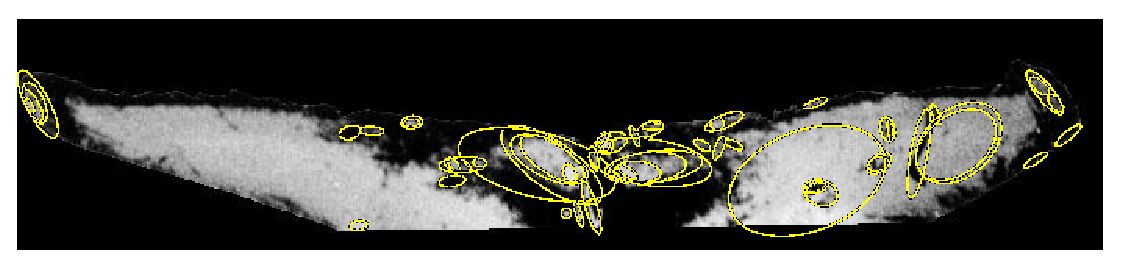
\includegraphics[width=4.0cm]{./Figs/mserTailA}}
%  \vspace{1.5cm}
 % \centerline{(a) Results 1}\medskip
\end{minipage}
%\hfill
\begin{minipage}[b]{0.48\linewidth}
  \centering
  \centerline{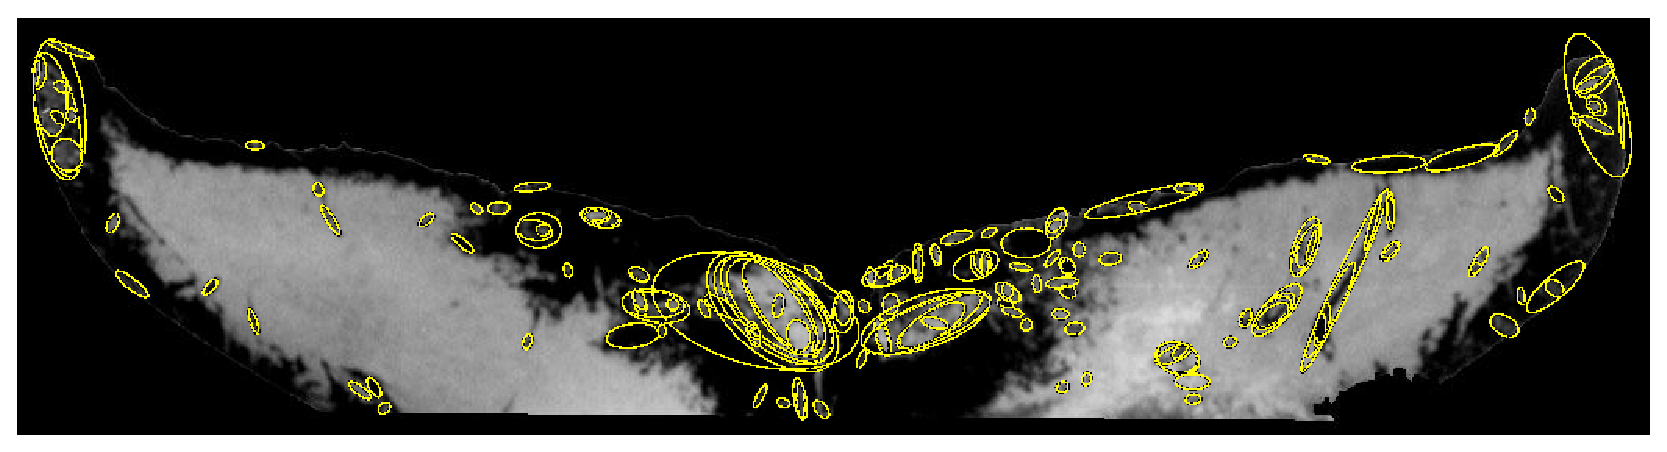
\includegraphics[width=4.0cm]{./Figs/mserTailB}}
%  \vspace{1.5cm}
%  \centerline{(b) Result 2}\medskip
\end{minipage}

\begin{minipage}[b]{.48\linewidth}
  \centering
  \centerline{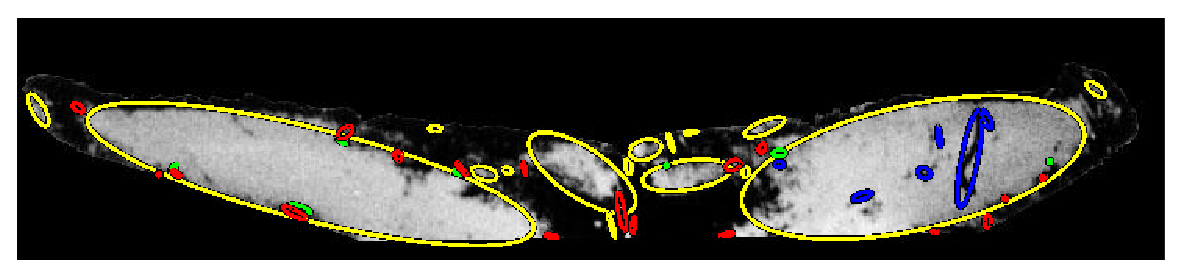
\includegraphics[width=4.0cm]{./Figs/dmsrTailA}}
%  \vspace{1.5cm}
 % \centerline{(c) Results 3}\medskip
\end{minipage}
%\hfill
\begin{minipage}[b]{0.48\linewidth}
  \centering
  \centerline{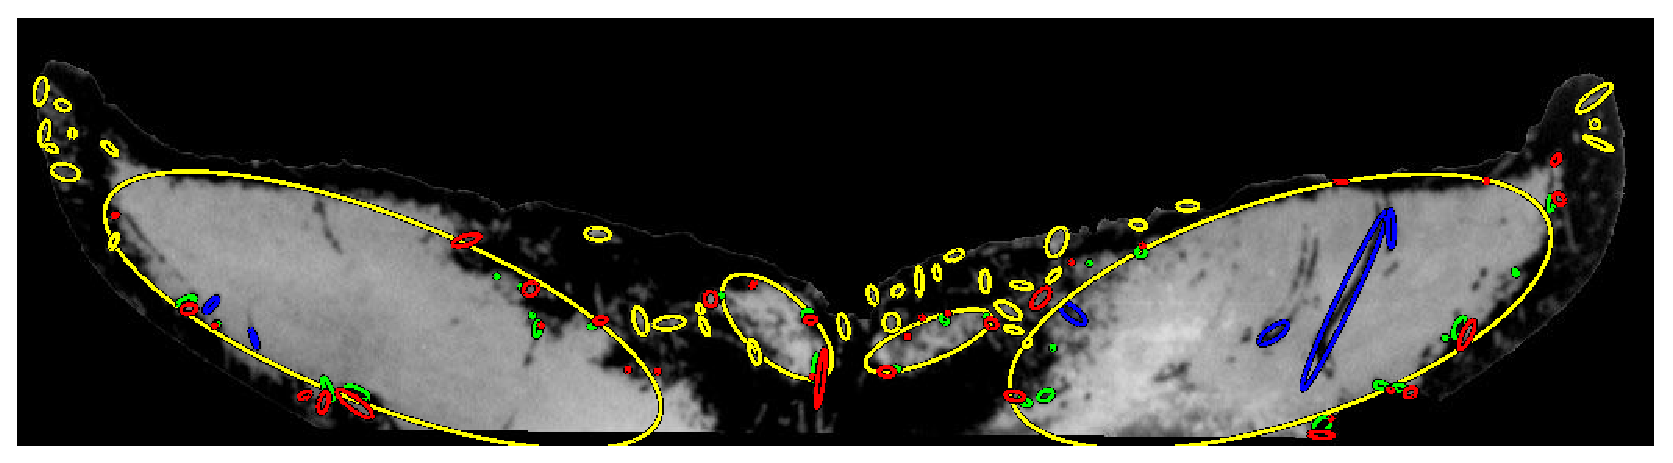
\includegraphics[width=4.0cm]{./Figs/dmsrTailB}}
%  \vspace{1.5cm}
%  \centerline{(d) Result 4}\medskip
\end{minipage}
 \vspace{-0.2cm}
\caption{Region detectors on two images of the tail of the same humpback whale. 
Top row: MSER, bottom row: DMSR.}
\label{fig:tails}
%
\end{figure}

%----------------------------------------------------------------
\begin{figure}[htb]

\begin{minipage}[b]{.24\linewidth}
  \centering
  \centerline{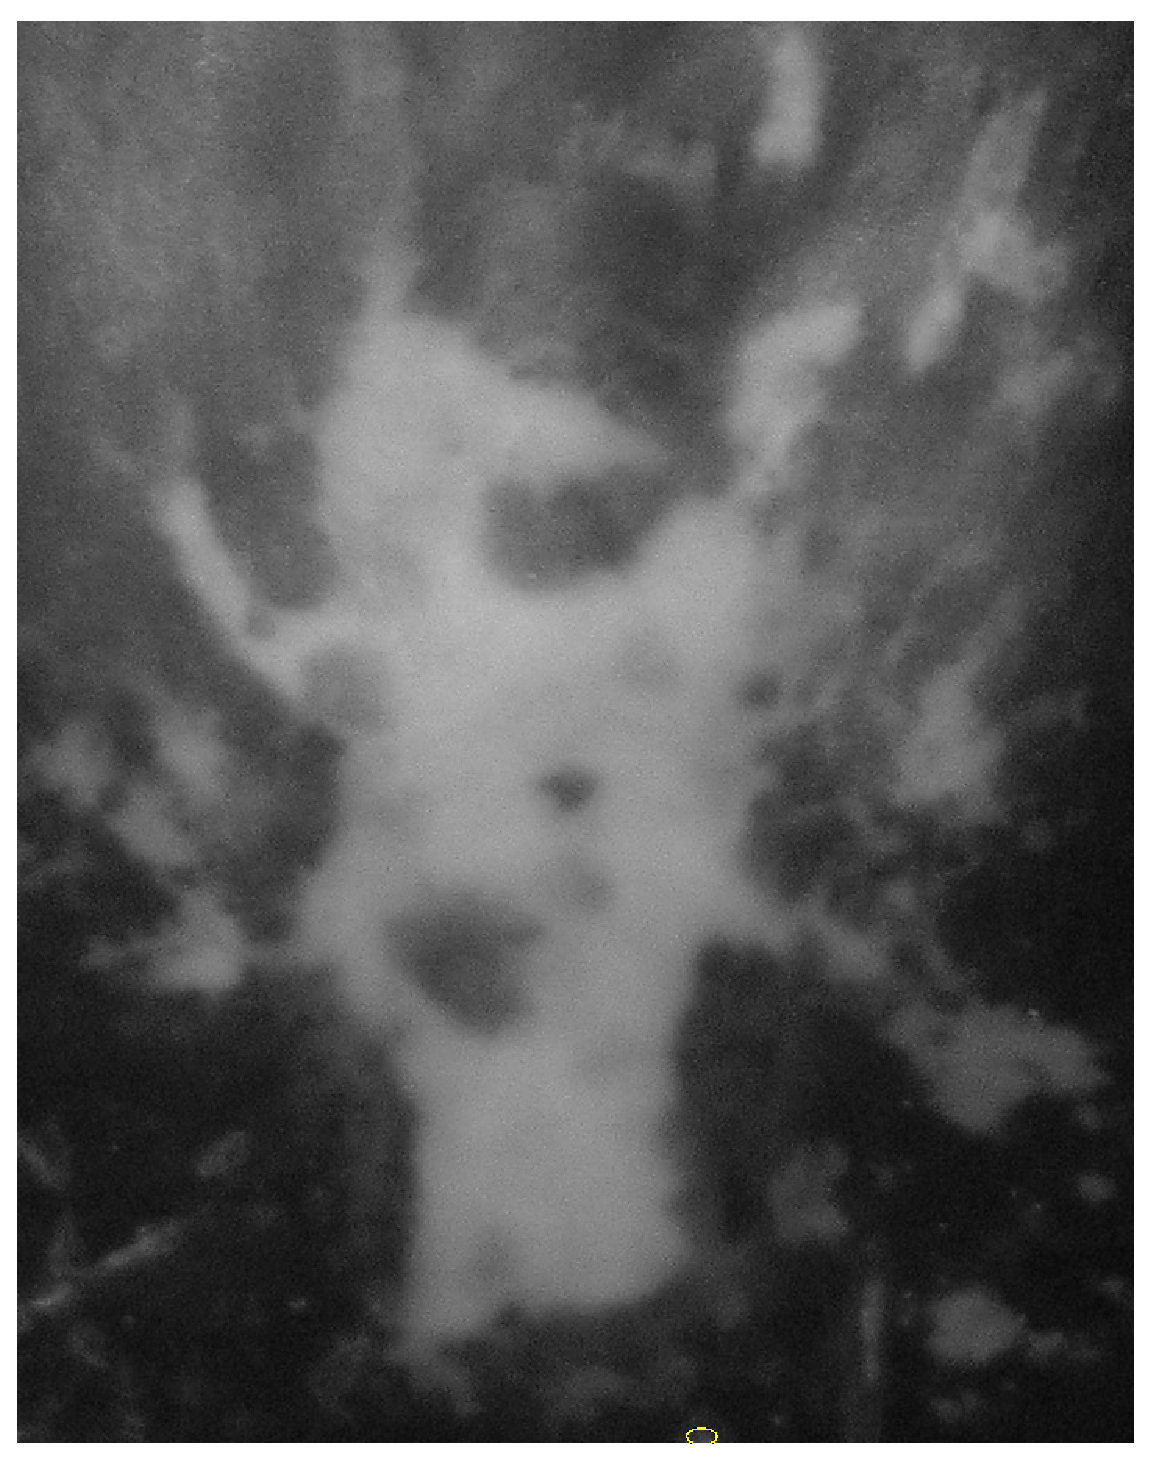
\includegraphics[height=2.0cm]{./Figs/mserLeatherbackA}}
%  \vspace{1.5cm}
  \vspace{-0.1cm}
   \centerline{(a)}\medskip
\end{minipage}
\hfill
\begin{minipage}[b]{0.24\linewidth}
  \centering
  \centerline{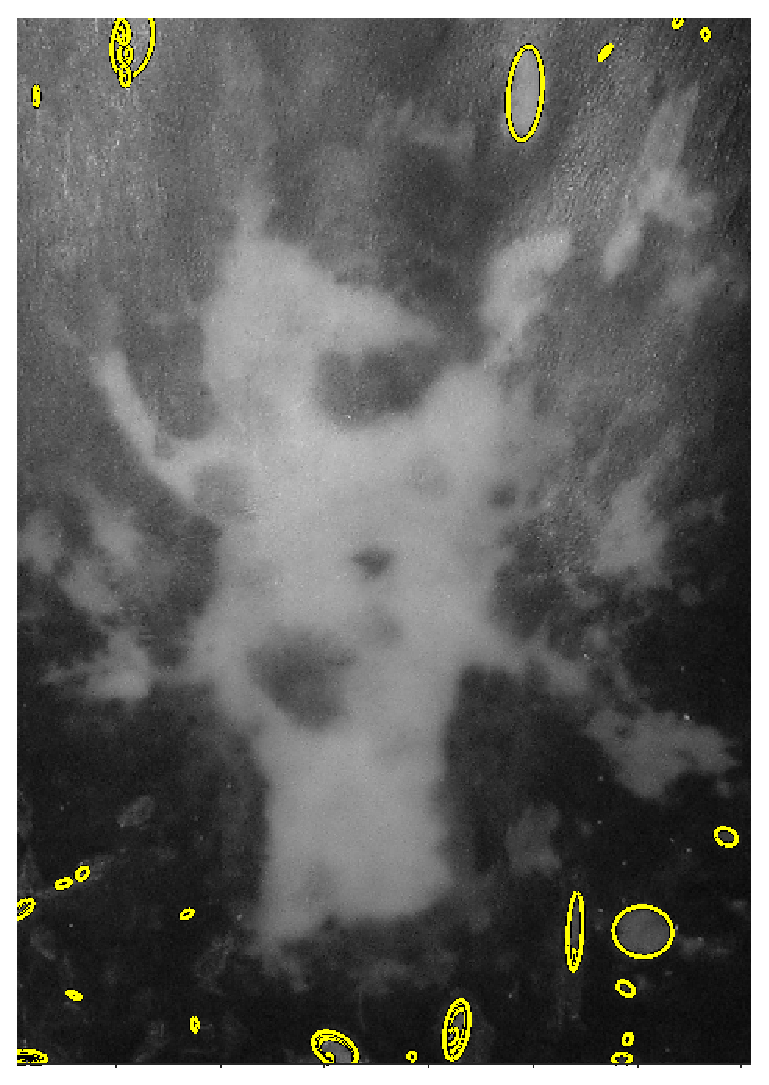
\includegraphics[height=2.2cm]{./Figs/mserLeatherbackB}}
  \vspace{-0.1cm}
\centerline{(b)}\medskip
\end{minipage}
\hfill
\begin{minipage}[b]{.24\linewidth}
  \centering
  \centerline{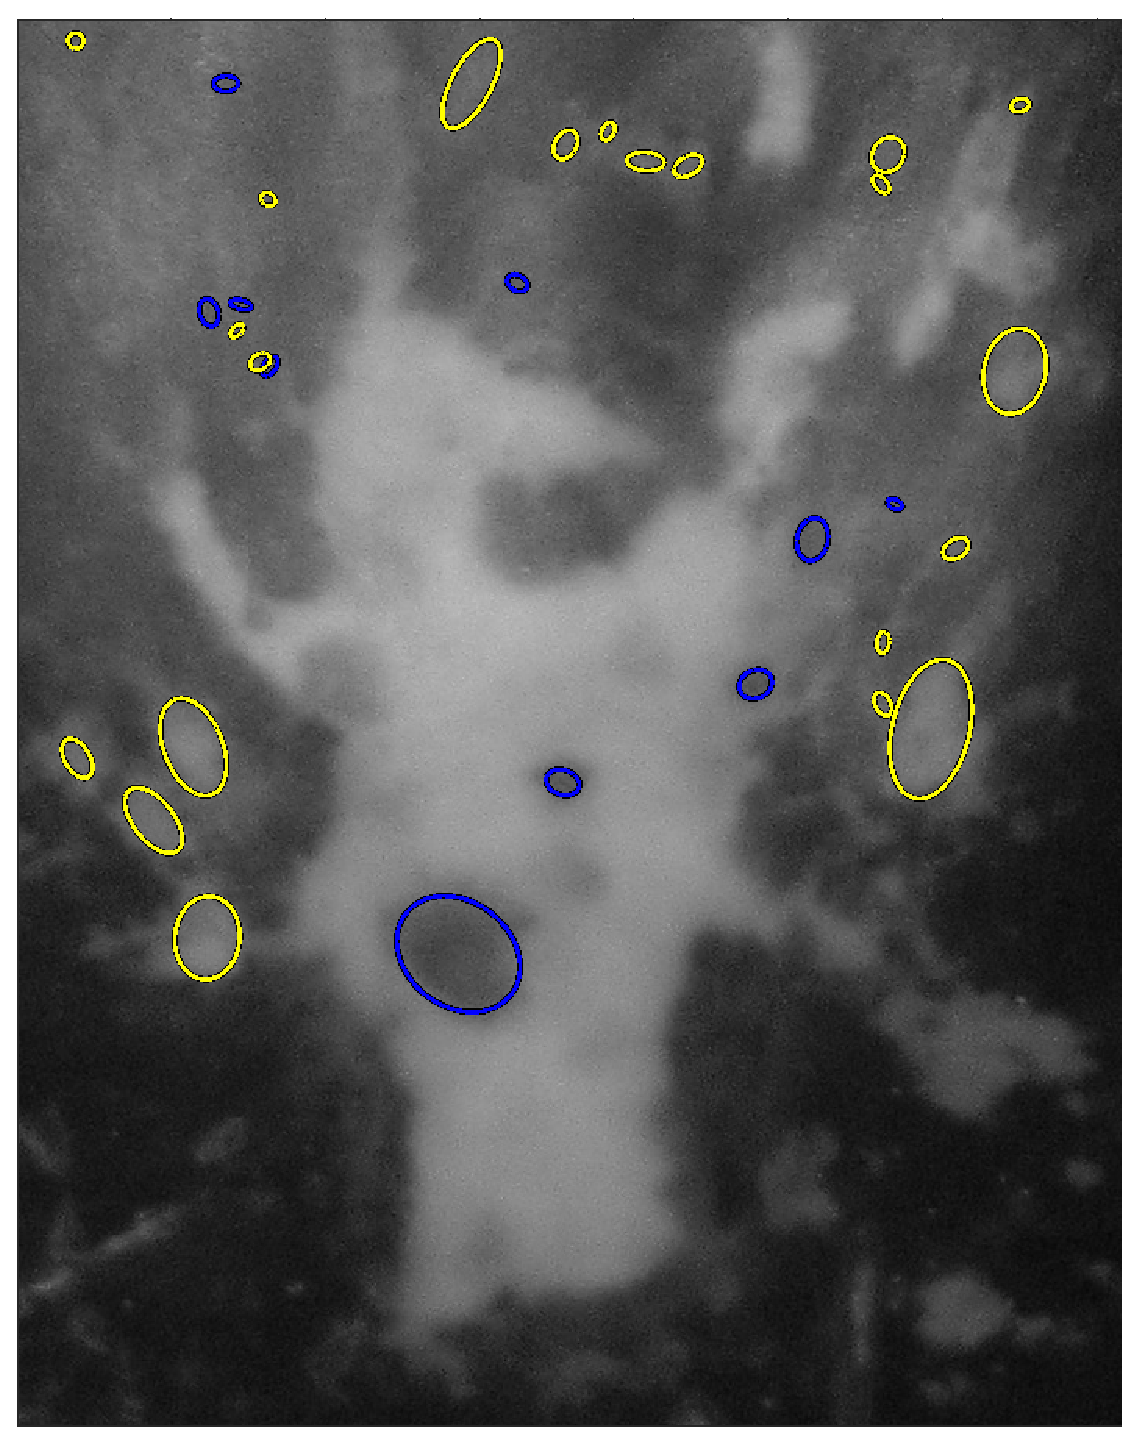
\includegraphics[height=2.0cm]{./Figs/dmsrLeatherbackA}}
  \vspace{-0.1cm}
\centerline{(c)}\medskip
\end{minipage}
\hfill
\begin{minipage}[b]{0.24\linewidth}
  \centering
  \centerline{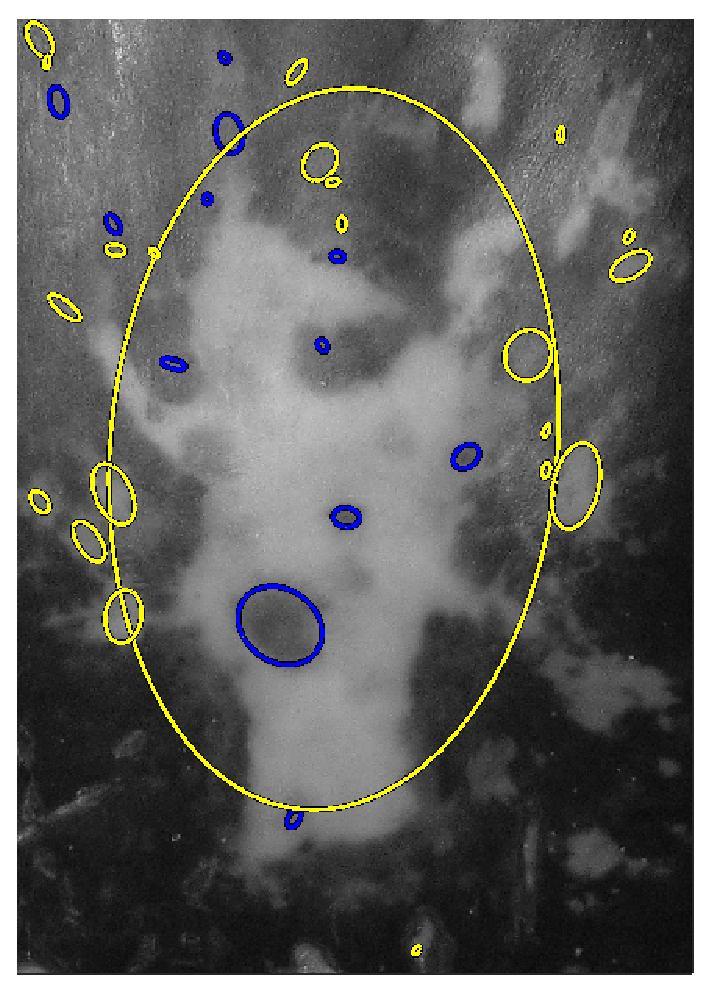
\includegraphics[height=2.2cm]{./Figs/dmsrLeatherbackB}}
  \vspace{-0.1cm}
 \centerline{(d)}\medskip
\end{minipage}

 \vspace{-0.5cm} 
\caption{Region detectors on two images of the pineal spot of the same leatherback turtle.
(a),(b): MSER, (c),(d): DMSR. }
\label{fig:turtle}
%
\end{figure}

There are not many evaluation benchmark datasets apart from the Oxford dataset, which is very small for nowadays standards: only $6$ test sequences and $48$ relatively low resolution images with known homographies and evaluation protocol, \cite{Mikolajczyk:2005}.  The {\em Freiburg dataset} contains $16$ base images, which give  $416$ transformed higher resolution images, \cite{FischerDB14}. Unlike the  naturally obtained images in the Oxford set, the Freiburg data have been generated by applying the transformations to each of the base images. This is done to de-tangle the transformations from the image content. Its main drawback is the lack of proper documentation of the transformation parameters. The {\em TNT dataset} contains several versions of few image transformed sequences with increasing resolution from $1.5$ MB to $8$ MB, along with very highly accurate homographies, compatible with the standard evaluation protocol, \cite{CorRos2013}. The TNT set contains only viewpoint transformation, focusing on evaluation robustness to resolution.


\subsection{Contributions}
\label{ssec:contr}

This paper makes the following contributions:\\
$\bullet$ Binarization algorithm, robust to image lighting and blur.\\
$\bullet$ DMSR salient regions detector for structure scenes. It is simpler and faster compared to MSSR, while the regions are also perceptually salient.\\
$\bullet$ DMSR gives much smaller and more stable number of regions compared to MSER, while having comparable or higher repeatability than MSER (for lighting, blur and increased resolution).\\
$\bullet$ More informative way of performance evaluation reporting in 3D for better insight in transformation covariance and higher resolution invariance.\\
$\bullet$ New open-source dataset 'OxFrei' combining good features of the Oxford and Freiburg datasets.The detector software is also open source.\\
$\bullet$ Demonstrated the potential of DMSR for scientific imagery analytics, mostly in the animal and plant biometric fields.



\section{Binary Salient Regions Detection}
\label{sec:binary}


\subsection{Binarization algorithm}
\label{ssec:binarize}


\section{Data-driven Morphology Salient Regions}
\label{sec:DMSR}


\section{Performance  Evaluation}
\label{sec:perf}

\subsection{Standard datasets}
\label{ssec:standart}

\subsubsection{Oxford dataset}
\label{sssec:oxford}
\subsubsection{Freiburg dataset}
\label{sssec:freiburg}
\subsubsection{Combined dataset}
\label{sssec:combined}
\subsubsection{TNT hi-res benchmark}
\label{sssec:tnt}

\section{CONCLUSIONS}
\label{sec:concl}




% To start a new column (but not a new page) and help balance the last-page
% column length use \vfill\pagebreak.
% -------------------------------------------------------------------------
%\vfill
%\pagebreak


\section{REFERENCES}
\label{sec:ref}


% References should be produced using the bibtex program from suitable
% BiBTeX files (here: strings, refs, manuals). The IEEEbib.bst bibliography
% style file from IEEE produces unsorted bibliography list.
% -------------------------------------------------------------------------
\bibliographystyle{IEEEbib}
\bibliography{icip2016}

\end{document}
